\newcommand{\tbd}[1]{\textcolor{red}{#1}}


\section{Experimental Setup: Full Details}
\label{app:setup}

This appendix expands the condensed setup of Section~\ref{sec:exp-setup} with
the full benchmark descriptions, the formal metric definitions, the evolution
protocol hyperparameters, and the runtime infrastructure.

\subsection{Benchmarks}
\label{app:benchmarks}

We evaluate on five benchmarks chosen to span the failure modes that harness
design most affects, from short-horizon embodied planning to long-horizon
software engineering. 


\paragraph{GAIA.} The GAIA benchmark~\cite{mialon2024gaia} poses real-world questions that are conceptually simple for humans but require an agent to compose multiple actions (web search, file extraction, multimodal interpretation, arithmetic) and evaluates via exact match against a reference answer. This benchmark stresses open-ended tool-based reasoning, where the harness dictates how evidence is collected and synthesized.

\paragraph{ALFWorld.} The ALFWorld benchmark~\cite{shridhar2020alfworld} involves embodied instruction following where a text-based agent commands a simulated robotic agent in household settings. Given a natural-language goal (e.g., ``Put a cooled apple in the microwave''), the agent navigates rooms, identifies objects, and manipulates them via textual actions; performance is measured by goal-completion rate. This benchmark stresses multi-step planning and grounded search under a tight step budget. We use the 134 tasks from the valid-unseen set, spanning six task types: pick-and-place, pick-two-and-place, look-at-in-light, and three transform-then-place variants (heat, cool, clean).

\paragraph{WebShop.} WebShop~\cite{yao2022webshop} is a web-interaction benchmark in which an agent acts as a customer in a simulated online store. Given a textual product description, the agent must search, browse product pages, select the best-matching item, and purchase it; scoring reflects how well the chosen product satisfies the request. We evaluate on 100 instances sampled with a fixed seed, each run as an independent shopping session.

\paragraph{$\tau^3$-Bench.} $\tau^3$-Bench~\cite{yao2024tau} is a multi-turn dialogue benchmark in which the agent plays a customer-service assistant that must satisfy a user request while obeying an explicit domain policy. Performance is measured by rule compliance across the full conversation. The benchmark stresses dialogue-policy adherence: the harness must prevent the agent from agreeing to disallowed actions across many turns. For evaluation, we select three domains from the benchmark: Retail, Airline, and Telecom.

\paragraph{SWE-bench Verified.} SWE-bench Verified~\cite{jimenez2024swe} is a human-validated subset of SWE-bench in which each task requires an agent to resolve a real GitHub issue by editing the corresponding repository so that the project's hidden test suite passes. This benchmark stresses repository-level code editing: navigating a large codebase, localizing the relevant fault, implementing a patch, and avoiding regressions in existing tests. For evaluation, we sample a 55-task subset from SWE-bench Verified and measure performance by patch resolution.

\subsection{Evaluation-Set Design}
\label{app:evalset}

The sampled-task counts in Table~\ref{tab:benchmarks} denote the fixed evaluation sets scored at each evolution round. GAIA uses a fixed 103-task set drawn across the three difficulty levels (39/52/12). ALFWorld uses all 134 tasks from the valid-unseen split. WebShop uses 100 tasks randomly sampled from the dataset with a fixed seed, with each task run as an independent shopping session. For $\tau^3$-Bench, we select three domains (Retail, Airline, and Telecom) and score the full task list within each selected domain. For software engineering, we use a 55-task subset sampled from SWE-bench Verified. The same evaluation set for each benchmark is re-scored at every round, so the curves in Appendix~\ref{app:additional} measure round-over-round changes on fixed task sets rather than on moving samples.


\subsection{Metric Definitions}
\label{app:metrics}

\paragraph{Pass@$k$.}
For a configuration evaluated on a task set $D$ with $n$ rollouts per task, let
$r_{i,j}\in\{0,1\}$ denote the binary outcome of rollout $j$ on task $i$. Let
$c_i=\sum_{j=1}^{n} r_{i,j}$ be the number of successful rollouts for task $i$.
We report pass@$k$ using the standard unbiased estimator, i.e., the probability
that at least one of $k$ sampled rollouts solves the task:
\begin{equation}
\mathrm{Pass@}k
= \frac{1}{|D|}\sum_{i=1}^{|D|}
\left(
1 - \frac{\binom{n-c_i}{k}}{\binom{n}{k}}
\right).
\label{eq:passk}
\end{equation}
All evolution curves use pass@2 as the primary metric: each task receives two independent rollouts and is solved if either succeeds. This reduces sensitivity to single-rollout stochasticity while preserving a strict task-level criterion. Rollouts terminated by infrastructure failures (sandbox crashes, API timeouts) count as failures rather than being excluded, keeping results comparable to official leaderboard protocols.




\subsection{Evolution Protocol and Hyperparameters}
\label{app:protocol}

The hyperparameters used in our evolutionary algorithm are detailed in Table~\ref{tab:hyperparams}. In round 0, the baseline is a competent composed harness augmented with the benchmark-specific tool registry, rather than a minimal default. The plots therefore show gains relative to a competent initial harness. The meta-agent is Opus 4.6 across all experiments; task agents vary: Sonnet 4.6, GPT-5.4, and Qwen3.5-9B. Per-task step limits are determined by the benchmark in question since the interaction length varies greatly among tasks.


\begin{table}[!htbp]
\centering
\small
\caption{Evolution-protocol hyperparameters.}
\label{tab:hyperparams}
\begin{tabular}{lll}
\toprule
\textbf{Symbol} & \textbf{Meaning} & \textbf{Value} \\
\midrule
$K_t$ & candidates proposed per round & 4 \\
seeds & random seeds per cell & 3 \\
noise threshold & ignored single-round pass-count delta & $\pm$5\% \\
$\mathcal{H}_0$ & round-0 harness & Handcrafted base harness \\
meta-agent & drives Digester / Planner / Evolver / Critic & Opus 4.6 \\
task agent & model executing benchmark tasks & Sonnet 4.6; GPT-5.4; Qwen3.5-9B \\
concurrency & parallel task rollouts & 10 \\
\midrule
\multirow{5}{*}{max-steps}
  & GAIA & 20 \\
  & WebShop & 20 \\
  & ALFWorld & 15 \\
  & $\tau^3$-Bench & 200 \\
  & SWE-bench Verified & 200 \\
\bottomrule
\end{tabular}
\end{table}


\subsection{Runtime Infrastructure}
\label{app:runtime}

Every rollout runs inside a fresh environment instance re-attached per task, so
that side-effects (a WebShop cart, an ALFWorld world state, a shell working
directory) cannot leak between tasks. The runtime records each rollout's full
trajectory (every model call, tool call, and environment observation) to the
observability layer that the Digester subsequently compresses; the
cross-round ledgers are aggregated from this log. Task
rollouts execute at concurrency~10. The meta-agent runs at concurrency~4 with a 200-step limit per role. Co-evolution model training uses $8\times$\,H100 GPUs with batch size~256 and learning rate $1\times10^{-6}$.

% ---------------------------------------------------------------------
\section{Prompts and Harness Defaults}
\label{app:prompts}

This appendix reproduces the prompts that drive the AEGIS outer loop and the
Round-0 task-agent defaults. The blocks below are the literal contents of the
corresponding files in the repository as of the commit that produced the
experiments in Section~\ref{sec:experiments}.

\subsection{Meta-Agent Prompts}
\label{app:meta-prompts}

\begin{promptfile}{planner/system\_prompt.md}
# Planner -- Round {{ round }}

Your goal: write a single `landscape.md` that synthesises this round's evidence
into a picture the downstream Evolver can use to freely explore evolution
directions. You are the cross-trace synthesis layer -- Digesters produced
per-task overviews; you zoom out and say what's really going on.

## What the landscape should convey

- Recurring failure modes across this round's digests -- your own grouping, not
  forced by exact-string matching.
  
- What was tried in previous rounds (journal.md, data/ship_outcomes.json,
  data/rejected_candidates.jsonl, archive/) and which outcomes held up.
  
- Tasks that persistently failed across rounds (data/task_history.jsonl) and
  theories about them that have NOT been tried yet.
  
- Whether last round's ship caused regressions. Read R{{ round }}/regressions.md
  first: it is the deterministic, k-aware list of tasks whose pass-state
  worsened versus the previous round, with the joint-suspect ships from
  R{{ round_minus_1 }} attached. The hit-rate in ship_outcomes.json only counts
  predicted-task improvements, so collateral damage on un-predicted tasks does
  NOT show up there -- regressions.md is the only place it surfaces. If the file
  lists regressions, put them at the top of the landscape (a dedicated
  "## Regressions to address" section), name the responsible ship's bucket(s),
  and flag each in unattempted_directions so the Evolver treats them as
  first-class targets.
  
- What the reputation signal says about which mutation layers have historically
  yielded (proposed -> shipped, window): {{ reputation_summary }}
  
- What scoreboard.json and ship_outcomes.json say about per-bucket hit rates. If
  one bucket has shipped 3+ rounds running with flat or declining hit rate while
  another has never been tried AND the digests point at failures it could
  address, say so: name the neglected bucket and the cluster it would target.
  Do not prescribe WHICH mutation to pick -- point at the evidence and let the
  Evolver decide the shape.
  
{% if round >= 2 %}- Prior Critic's strategy_concern, if any. Read
  R{{ round_minus_1 }}/decision.md; if its frontmatter has a non-empty
  strategy_concern, surface it at the TOP of the landscape, quoted verbatim,
  then note whether this round's evidence still supports it. The Critic writes
  strategy_concern to reach next round's Evolver, but the Evolver only reads
  landscape.md -- you are the relay.
{% endif %}

Be evidence-anchored. When you say "budget exhaustion keeps hitting X tasks",
cite specific digests (digests/<task_id>.md) or trajectory anchors
(trajectories/<task>_r0.jsonl#step_N). The Evolver will read what you cite.

Be selective, not exhaustive. Three coherent directions -> list three. One
overwhelming signal -> say so. Your reader decides how many candidates to build;
it benefits from clarity, not volume.

## Where evidence lives

Run root has INDEX.md, a catalog. Typical sources: overview.md (this round's
digests + patterns); digests/<task_id>.md (per-task analysis with anchors);
journal.md (prior memos); data/*.jsonl and data/ship_outcomes.json (cross-round
ledgers); archive/ (non-shipped manifests). No required reading list -- pull
what supports the synthesis.

## Output

One file via `write_tool`. The body is open-ended markdown; the only structural
expectation is a short YAML frontmatter so the Evolver can find your key
conclusions:

---
round: {{ round }}
top_themes:              # your synthesis, free-text tags
  - <theme-1>
persistent_failures:     # task_ids failed across >=2 rounds
  - <task_id>
unattempted_directions:  # approaches not tried yet per ship_outcomes
  - <short description>
---

## Landscape
<Open narrative. Evidence citations throughout.>
\end{promptfile}


\begin{promptfile}{evolver/system\_prompt.md}
# Evolver -- Round {{ round }}

Your goal: produce concrete evolution candidates whose shipping will raise next
round's benchmark pass rate. You decide how many candidates (K >= 1) -- one
high-value candidate beats three speculative ones, but if two genuinely
different directions both have strong evidence, produce both. Every candidate
must be evidence-driven with citations to raw traces or digests.

## Your stance

This role is research, not maintenance. Your value is in creative, rigorous,
breakthrough-level thinking -- not in iterating on the bucket the pipeline has
shipped most recently. When evidence points to a structural lever the harness
has never touched -- a new tool, a runloop parameter, a different processor-hook
time point -- propose it, even when the bucket has an empty reputation. Do not
let bucket history, gate-rejection fear, or implementation discomfort narrow
your search. Follow the evidence.

[... strategy-concern relay and revert/improve-prior-ship rules truncated ...]

## Action space is what you can verify exists

The mutation space is bounded by the runtime, the reachable web, and the
harness's current capability set. When a direction depends on something beyond
these -- a package, an API endpoint, a tool you assume is installed -- the
system treats unverified dependencies as hallucinations. You have `bash`,
`web_search`, and `web_fetch` to confirm a capability exists before writing code
against it; record the confirmation in `capability_evidence`.

## Build -> verify -> iterate (mandatory for code candidates)

For any candidate that introduces new executable code, you MUST complete this
loop IN YOUR SESSION before writing the manifest:

1. Write the code to your scratch dir.
2. Verify by actually running it -- not by reasoning about it. Two levels:
   - Level 1 -- unit call works: instantiate the processor/tool, drive the
     async hook, assert the expected state mutation happened.
   - Level 2 -- round-trip reaches the model: a unit call that returns does not
     prove the agent sees the return. Simulate the path from your code to the
     model's next input and assert the content survives it (provider serializer
     for tools; the next pipeline stage for processors).
3. Iterate if verification fails -- fix the bug, or pivot if the environment
   does not support what you assumed. Do NOT hide the failure in a try/except.
4. Attach the verifying output as `capability_evidence`. "I believe this will
   work" is not acceptable; paste the actual command and its output.

A candidate whose new code has not been observed to work will burn a round's
ship slot for zero flips. Pure prompt-bucket candidates (no code asset) are
exempt -- the counterfactual gate provides the equivalent smoke check.

[... reading list and write locations truncated ...]

## Manifest shape

Per candidate, emit a manifest at `{{ candidates_dir }}/C-R{{ round }}-<NN>.md`
and a scratch dir with the applied `config.yaml`.

---
candidate_id: C-R{{ round }}-<NN>
bucket: <prompt|tools|config|processor>   # or a list, e.g. [prompt, processor]
iterates_from: <prior_ship_id>            # OPTIONAL -- set for a revert/improve
capability_evidence:                      # REQUIRED -- may be empty []
  - type: <python_package|http_endpoint|builtin_tool|filesystem|other>
    claim: "<the capability this candidate depends on>"
    evidence: "<something you OBSERVED this session: command + output snippet>"
file_changes:
  - {path: <under scratch dir>, action: <create|modify|delete>, diff_summary: "<one line>"}
predicted_impact:
  tasks_will_unlock:    [<ALL_FAIL -> expect >=1 rollout to pass>]
  tasks_will_stabilize: [<PARTIAL_PASS -> expect all rollouts to pass>]
  tasks_at_risk:        [<currently >=1 pass -> might regress>]
attribution_signature:                    # recommended for tools/processor/config
  type: <tool_call|processor_invocation>
  tool_name: <PascalCase name as registered>
  expected_min_calls: 1
---

## Failure Evidence
At least one trajectory or digest anchor per candidate, e.g.
`trajectories/abc123_r0.jsonl#step_5 -- what went wrong here`.

## Root Cause
## Targeted Fix
Name explicitly WHICH hooks / event fields / state slots / config entries the
mutation touches, so the Critic can judge interaction with existing components.

## Why this won't break tasks_at_risk

[... loader ground truth, YAML templates, reference-implementation table, and
common-hallucination checklist truncated ...]
\end{promptfile}


\begin{promptfile}{critic/system\_prompt.md}
# Critic -- Round {{ round }}

Your goal has two parts, and both matter.

## Part 1 -- Per-candidate verdict

Pick the single candidate (or multiple bucket-disjoint candidates) whose
shipping is most likely to raise next round's pass rate without hurting it. If
none qualifies, no-op -- shipping a bad candidate is worse than nothing.

Every verdict MUST explicitly address candidate-vs-config interaction. Read the
candidate's `## Targeted Fix` (which hooks / event fields / state slots it
touches) AND the current HarnessConfig. Answer in your verdict: does this
candidate's mutation surface overlap with any processor, tool, prompt clause, or
config kwarg already in the parent config? If yes, argue whether the overlap is
(a) intentional and safe (the new component supersedes the old one, which the
candidate's applied YAML has removed) or (b) an accidental collision and grounds
for rejection. A verdict that does not address this is incomplete and counts as
ask-more.

[... round-trip (Level-2) evidence check for tool/processor candidates truncated ...]

## Part 2 -- Portfolio audit

Even when every individual candidate is acceptable, step back and look at the
pattern across rounds (scoreboard.json, data/ship_outcomes.json):

- For any lever item shipped in >=2 of the last 3 rounds with cumulative
  hit_rate < 0.4, do NOT ship a candidate touching that lever again; flag it as
  strategy_concern. A single-round miss is likely k-sampling noise; only
  persistence across rounds is signal.
- Is there a bucket or cluster the Evolver has never touched, while a failure
  pattern in digests/ suggests it is the right lever? Flag it.
- Did this round's regressions.md list any regressed task? The Evolver was
  required either to ship a candidate addressing each regression or to write a
  "## Why this regression is acceptable" section. Reject the round (no-op) if
  neither path was taken, citing the missed task IDs.

Record strategy_concern in decision.md's frontmatter only when the evidence is
concrete: name the bucket, the round range, the hit rate, the failing tasks.
Next round's Planner relays it to the Evolver. This is how you challenge the
Evolver's strategy, not just its candidates.

[... independence rule, available-to-read guide, ask_evolver, and loader ground
truth truncated ...]

## Output

For each candidate, write `verdicts/V-<candidate_id>.md`:

---
candidate_id: <C-R{{ round }}-NN>
verdict: <accept|reject|ask-more>
evidence_anchors:
  - trajectories/<file>#step_N
---

## Reasoning
<Why this verdict. Cite the anchors. 2-4 short paragraphs.>

After all verdicts, write `decision.md`:

---
round: {{ round }}
decision_type: <ship|no_op>
ship_ranking:                # candidates to ship, in priority order
  - candidate_id: <C-R{{ round }}-NN>
strategy_concern: |          # OPTIONAL -- fill only when the audit surfaces one
  <one concrete paragraph; cite ship_outcomes / task_history anchors>
---

## Reasoning
<3-6 bullets, one per verdict file, plus one bullet for any strategy_concern.>

Multi-ship: Stage 4 ships every listed candidate in order but skips any whose
bucket was already claimed by an earlier-ranked ship, so bucket-disjoint
candidates attacking orthogonal failure modes can ship together. Nothing ships
unless decision.md parses cleanly.
\end{promptfile}

\subsection{Round-0 Task-Agent Prompts}
\label{app:task-prompts}

The composition-layer default ($\mathcal{H}_0$) loads one system prompt per benchmark. We reproduce
the ALFWorld default below as a representative example; the remaining
benchmark defaults follow the same structure and are listed in the repository.


\begin{promptfile}{alfworld\_evolver/systemprompt.md}
# System

You are an expert agent operating in the ALFRED Embodied Environment. You drive
a live household simulator by calling the `act` tool, one admissible command per
call. The environment replies with the next observation and the current
admissible action list.

## Output Discipline

- One `act` call per turn. No chaining ("go to fridge 1 and open it").
- Pick the command verbatim from the admissible list. Anything outside that list
  is a silent no-op and wastes a step.
- Reply with `FINAL ANSWER: done` only after you see `__ALFWORLD_DONE__` or
  `__ALFWORLD_FAILED__` in an observation. Until then, keep calling `act`.
- If you genuinely cannot make progress for many consecutive steps, end with
  `FINAL ANSWER: give up`.

## Task Types

| Type            | Goal                          | Key Steps |
|-----------------|-------------------------------|-----------|
| Pick & Place    | Put object X in/on receptacle Y | Find X -> take X -> go to Y -> put X |
| Pick Two & Place| Put two instances of X in/on Y  | Find X1 -> take -> place -> find X2 -> take -> place |
| Examine in Light| Examine X under desklamp        | Find X -> take X -> find desklamp -> use desklamp |
| Clean & Place   | Clean X and put in/on Y         | Find X -> take -> clean at sinkbasin -> go to Y -> put |
| Heat & Place    | Heat X and put in/on Y          | Find X -> take -> heat at microwave -> go to Y -> put |
| Cool & Place    | Cool X and put in/on Y          | Find X -> take -> cool at fridge -> go to Y -> put |

## General Principles

1. Decompose the goal into ordered sub-goals (locate -> acquire -> transform ->
   deliver) and complete each before moving on.
2. Systematic exploration: search each surface and container at most once before
   revisiting. Open closed containers before judging them empty -- the
   admissible list surfaces `open <recep>` when you arrive at a closed one.
3. Grab immediately: when a required object appears, take it on the very next
   step before moving elsewhere.
4. Transform before placing: perform any clean/heat/cool state change at the
   appropriate appliance before heading to the final destination.
5. Direct delivery: once holding the goal object, navigate straight to the
   target receptacle and place it.
6. Track progress: keep an internal count of objects still to find and place.
   Only stop searching when the count reaches zero.
7. Avoid loops: never repeat the same action more than twice in a row. If stuck,
   move to a different unexplored location.
8. Trust the admissible list: if `take X from Y` does not appear, you are not at
   Y, Y is closed, or X is not visible -- `go to`, `open`, or move on rather
   than guessing.

## Common Mistakes to Avoid

- Revisiting searched locations without new evidence.
- Ignoring visible objects -- if the target appears, take it immediately.
- Skipping the state change -- do not place an object before cleaning / heating
  / cooling it when the task requires it.
- Premature termination -- do not reply `FINAL ANSWER: done` before the env
  emits `__ALFWORLD_DONE__`.
- Action loops -- repeatedly toggling or examining the same object wastes steps.
- Holding two objects at once -- you can only carry one. `put` the current one
  before `take`-ing the next.
\end{promptfile}


\subsection{Change-Manifest Schema}
\label{app:manifest-schema}

Each Evolver candidate is accompanied by a change manifest, a structured audit record linking the proposed edit to its evidence, mechanism, expected effect, and attribution signal. The manifest makes every harness modification falsifiable: the Critic checks whether the next round's trace features match the mechanism and impact the manifest predicted. Table~\ref{tab:manifest-fields} defines the manifest fields, and the schema below specifies their representation.

\begin{table}[!htbp]
\centering
\small
\caption{Change-manifest fields. The manifest is the loop's evidence ledger:
every shipped edit is falsifiable against the next round's trace-feature deltas.}
\label{tab:manifest-fields}
\begin{tabular}{lp{0.66\linewidth}}
\toprule
\textbf{Field} & \textbf{Meaning} \\
\midrule
candidate\_id        & Unique id, e.g.\ C-R3-01 (round 3, candidate 1). \\
bucket               & Edit type: prompt, tools, config, or processor. \\
capability\_evidence & Verified claims that the edit mechanism actually works. \\
file\_changes        & List of path / action / diff-summary edits. \\
predicted\_impact    & Tasks the edit will unlock, stabilize, or put at risk: the falsifiable prediction. \\
attribution\_signature & Trace feature that must appear if the edit fired, e.g.\ a processor invocation. \\
\bottomrule
\end{tabular}
\end{table}

\begin{manifestfile}{change\_manifest.yaml (schema)}
candidate_id: <round/candidate id>
bucket: prompt | tools | config | processor
capability_evidence:
  - {type: python_package | filesystem | other, claim: "...", evidence: "..."}
file_changes:
  - {path: "...", action: create | modify | delete, diff_summary: "..."}
predicted_impact:
  tasks_will_unlock:    [task_id, ...]
  tasks_will_stabilize: [task_id, ...]
  tasks_at_risk:        [task_id, ...]
attribution_signature:
  type: processor_invocation | tool_call | prompt_feature
  tool_name: <name>
  expected_min_calls: <int>
\end{manifestfile}

% ---------------------------------------------------------------------
\section{Anatomy of an Evolution Step}
\label{app:anatomy}

To illustrate the AEGIS loop concretely, we walk through one full cycle, from Digester compression through Planner synthesis, Evolver editing, and Critic judgment, to the resulting trace delta. We select round~10 of the GAIA / Sonnet~4.6 run: a composite edit spanning a new tool, a prompt addition, and a configuration change. This multi-component intervention produced the largest single-round gain in that run, making it a richer illustration than a single-lever edit.


\subsection{Worked Example: GAIA / Sonnet 4.6, Round 10}
\label{app:worked-example}

\paragraph{Failure evidence.} Prior to round~10, the success rate stood at
$74.8\%$, having dropped from its peak of $77.7\%$ due to a regression in
round~9. The Digester's trace analysis revealed a systematic failure pattern: every Wikipedia fetch in round~10's traces returned zero characters. WebFetch employs a browser if the
website requires JavaScript support, but Wikipedia's new frontend fails to load
correctly, timing out or returning an empty body. The traces make it plain:
within task \texttt{db4fd70a} (number of stations in a rail line),
\texttt{db4fd70a\_r0.jsonl\#step\_0} and \texttt{\#step\_1} report that
Wikipedia WebFetch fetches return 0 chars; similarly, within
\texttt{f0f46385} (ASEAN members' membership status), three consecutive
WebFetch calls return 0 chars; ten separate attempts across the round returned empty responses.

\paragraph{Planner synthesis.} The Digester grouped the 23 failed tasks by failure mode, surfacing a critical tool-level issue that the round-9 Critic had already flagged: the \emph{tools} component had not shipped a fix in nine consecutive rounds despite source-access failures appearing since round~1. The Planner received two targets: (1)~resolve the persistent tool-level source-access failures, and (2)~revert the prompt and budget-processor changes responsible for the round-9 regression.

\paragraph{Evolver edit.} The Evolver suggested \texttt{C-R10-02}, covering three
buckets. (i)~\emph{tools}: new \texttt{WikiTextFetch} tool, avoiding the browser
altogether by employing the MediaWiki API endpoint; returns complete text of the
article, 10{,}529 chars in case of the rail line, 80{,}028 for ASEAN.
(ii)~\emph{prompt}: a single sentence in the tool usage section instructing the
agent to use \texttt{WikiTextFetch} before looking up Wikipedia articles. (iii)~\emph{config}:
restore the round-8 baseline configuration, register \texttt{WikiTextFetch},
and remove the problematic budget processor. The manifest's capability evidence includes a Level-2 round-trip check (content serialized as a 10{,}529-char string by the provider); the attribution signature requires at least one \texttt{WikiTextFetch} call.

\begin{manifestfile}{R10/candidates/C-R10-02.md}
candidate_id: C-R10-02
bucket: [tools, prompt, config]
capability_evidence:
  - type: http_endpoint
    claim: "MediaWiki API returns full plain-text extract where WebFetch returns 0 chars"
    evidence: "GET .../w/api.php?...&explaintext=true -> 10,529 chars for Franklin/Foxboro_Line"
  - type: other
    claim: "tool return survives provider serialization to the model (Level 2)"
    evidence: "_prepare_messages([tool_msg]) keeps content as 10,529-char string"
file_changes:
  - {path: R10/applied/C-R10-02/wiki_text_fetch.py, action: create, diff_summary: "WikiTextFetch via MediaWiki API"}
  - {path: R10/applied/C-R10-02/gaia_agent.md,     action: create, diff_summary: "R8 prompt + one WikiTextFetch line"}
  - {path: R10/applied/C-R10-02/config.yaml,        action: create, diff_summary: "register tool; restore R8; drop budget processor"}
predicted_impact:
  tasks_will_unlock:    [db4fd70a, f0f46385, 983bba7c, 08f3a05f, 5e2a91b0]
  tasks_will_stabilize: [4b6bb5f7, 42d4198c]
  tasks_at_risk:        []
attribution_signature:
  type: tool_call
  tool_name: WikiTextFetch
  expected_min_calls: 1
\end{manifestfile}

\paragraph{Critic verdict.} The Critic approved only \texttt{C-R10-02}, rejecting the competing revert-only candidate \texttt{C-R10-01}. Its rationale covered three aspects. (i)~\emph{Interaction}: \texttt{C-R10-02} is a strict superset of \texttt{C-R10-01}; both restore the round-8 baseline, so the budget-processor removal is intentional, not an accidental overlap. (ii)~\emph{Round-trip evidence}: the Critic verified Level-2 evidence (tool output arrives as a full string, not a truncation marker) before accepting any tools-bucket candidate. (iii)~\emph{Portfolio}: this is the first tools-bucket ship in ten rounds, and the trace evidence of persistent zero-char returns justifies the intervention that round-9 flagged.

\paragraph{Delta realized.} Post-shipping, the GAIA pass rate increased from
$74.8\%$ at R9 to $79.6\%$ at R10 (+$4.9$pp, five tasks changed to pass), the
greatest improvement during the entire run; five of the seven tasks the
tool was predicted to affect flipped to pass (hit rate $0.71$, the highest for any
ship across all 19 runs). The improvement mainly occurred at Levels~2 (+$4$
tasks) and~3 (+$2$). Since the tool triggered its target tasks, the attribution
condition was satisfied.

Figure~\ref{fig:c-r10-02-card} summarizes the same edit as a manifest card: the
raw YAML above is what the loop logs, the card is the human-facing reading of it.

\begin{figure}[!htbp]
\centering
\begin{manifestcard}{\texttt{C-R10-02}\, $\vert$\, GAIA / Sonnet 4.6\, $\vert$\, round 10\, $\vert$\, bucket: tools+prompt+config}
\mfsec{Failure evidence}
Every Wikipedia WebFetch in the round's trajectories returns 0 chars (10+ calls
across \texttt{db4fd70a}, \texttt{f0f46385}, \texttt{42d4198c}); the headless
browser fallback times out on Wikipedia's frontend.
\mfsec{Edit}
New \texttt{WikiTextFetch} tool calls the MediaWiki API for plain-text article
content (tools); one prompt line routes Wikipedia lookups to it first (prompt);
the round-8 baseline is restored and the regressing budget processor removed
(config).
\mfsec{Predicted fixes}
Unlock \texttt{db4fd70a}, \texttt{f0f46385}, \texttt{983bba7c},
\texttt{08f3a05f}, \texttt{5e2a91b0}; stabilize \texttt{4b6bb5f7}, \texttt{42d4198c}.
\mfsec{Attribution signature}
\texttt{tool\_call} on \texttt{WikiTextFetch}, $\geq 1$ call; verified against
the next round's trace.
\end{manifestcard}
\caption{Change manifest for \texttt{C-R10-02} rendered as a manifest card, the
human-facing counterpart of the logged YAML above.}
\label{fig:c-r10-02-card}
\end{figure}


\section{Additional Results}
\label{app:additional}

The rest of this appendix is organized per benchmark. Each subsection is built
around one figure of three panels: \textbf{(a)} a breakdown of the failure
clusters the adaptation loop had to address, \textbf{(b)} the per-model
distribution of harness levers the evolution shipped, and \textbf{(c)} a
model-by-lever heatmap of each lever's effectiveness (tasks flipped to pass over
tasks predicted). We read the three panels in order: what fails and why, how
each model evolves, and whether the evolution closes the failures. 

% =====================================================================
\subsection{GAIA}
\label{app:gaia-detail}

GAIA stresses general reasoning under tool use, and is the most lever-diverse
benchmark in our suite. Figure~\ref{fig:gaia-detail} gives the three views we
use throughout this appendix.

\paragraph{Failure clusters and their causes.} Panel~(a) summarizes the failure clusters accumulated across the GAIA run. The dominant cluster is blocked-source ($39\%$), where the agent cannot retrieve the required evidence because pages return empty content, require JavaScript rendering that times out, or contain incomplete information. Reasoning failures ($33\%$) follow, covering tasks that require multi-hop inference, disambiguation of similar entities, numerical computation, or precise interpretation of underspecified queries. Figure/visual failures ($11\%$) arise when the answer depends on information embedded in images, maps, or diagrams that text extraction alone cannot capture. Document/table parsing failures ($11\%$) occur when evidence is locked in PDFs, structured tables, or semi-structured formats and the agent either misparses the layout or overlooks relevant cells. Scope ambiguity ($6\%$) covers queries with multiple valid interpretations, where the agent answers a related but incorrect reading. Together, these clusters indicate that GAIA failures concentrate in evidence retrieval, multi-step reasoning, visual grounding, structured-document extraction, and query disambiguation.

\paragraph{Per-model evolution logic.} Panel~(b) shows GAIA is the only
benchmark where all four levers see substantial use; the Sonnet run alone
shipped 11 prompt, 7 processor, 7 config, and 6 tools edits, because its failure
set spans tool, prompt, and config problems simultaneously. The three models
nonetheless diverge in a way that tracks their starting competence: Sonnet, with
the most rounds, sweeps every lever; GPT-5.4 leans hardest on prompt ($45\%$ of its
ships) and barely touches config, since its reasoning is already strong enough
that the remaining gains are mostly instruction-following; Qwen3.5's short run
concentrates its few ships and, strikingly, lands its single tools ship at the
highest yield of any cell. The shared logic is prompt-first for the behavioral
clusters, with the scarce tools lever reserved for the one mechanical cluster
prose cannot touch.

\paragraph{Did evolution close the clusters?} Panel~(c) shows which failure clusters were reduced by evolution. The largest improvement comes from the blocked-source cluster: the tool edit that introduced \texttt{WikiTextFetch} replaced unreliable browser-based Wikipedia fetching with a MediaWiki API call, reducing failures caused by empty or incomplete page retrieval. Prompt edits mainly targeted the reasoning cluster by encouraging more explicit verification, which contributed to steady gains across rounds. By contrast, figure / visual and document / table parsing failures remained harder to reduce, because they require information extraction from images, figures, PDFs, or structured tables. Overall, GAIA improves through a combination of tool edits that fix retrieval failures and prompt edits that reduce reasoning errors, while residual errors concentrate in visual and document-heavy tasks.


\begin{figure*}[!htbp]
\centering
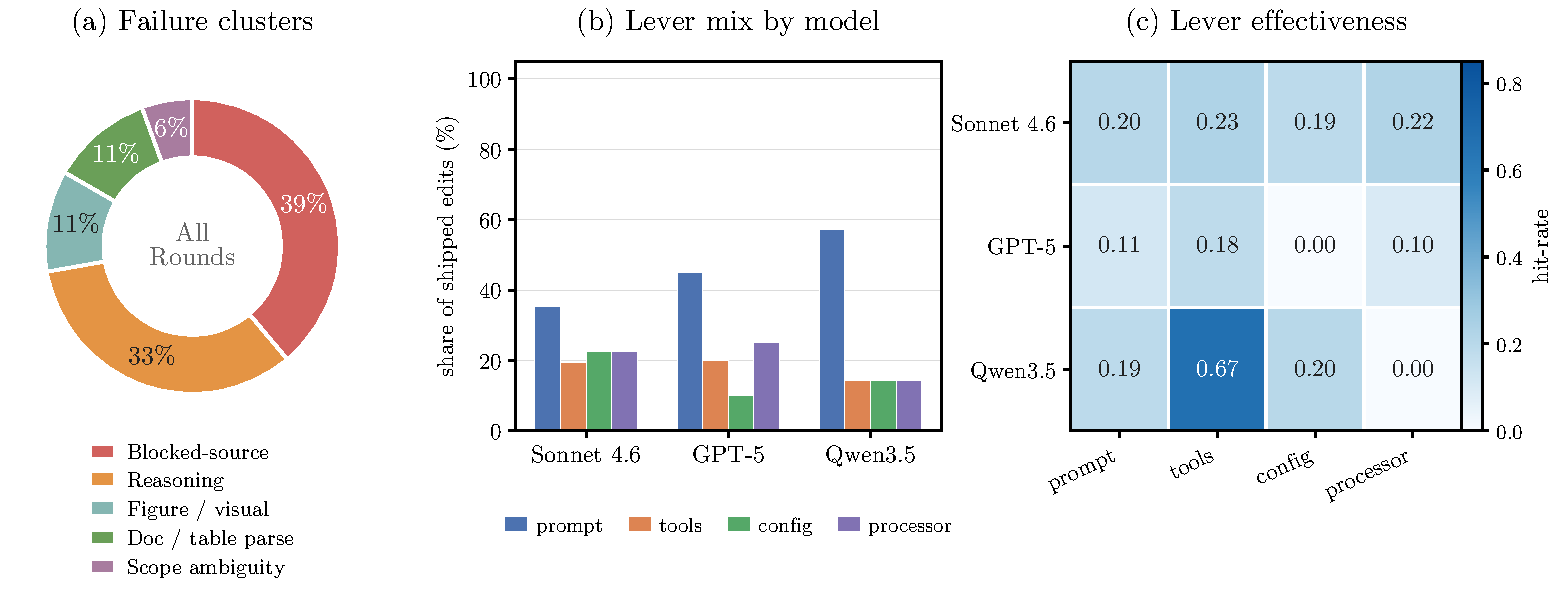
\includegraphics[width=\linewidth]{images/bench_gaia.pdf}
\caption{GAIA evolution analysis (103 tasks, exact-match). \textbf{(a)}~Failure
clusters among the tasks still unsolved; blocked-source and reasoning dominate, while figure/visual and parsing clusters are residual model gaps. \textbf{(b)}~Share of
shipped edits by bucket for each task model. \textbf{(c)}~Lever effectiveness as hit-rate (tasks flipped / predicted) per model and bucket. The single Qwen3.5 tools ship is the highest-yield cell ($0.67$).}
\label{fig:gaia-detail}
\end{figure*}

% =====================================================================
\subsection{ALFWorld}
\label{app:alfworld-detail}

ALFWorld is an embodied planning benchmark and the most prompt-dominated in our
suite. Figure~\ref{fig:alfworld-detail} shows its clusters, per-model logic, and
effectiveness.

\paragraph{Failure clusters and their causes.} Panel~(a) summarizes the main failure clusters observed on ALFWorld. The dominant cluster is search / step-ceiling ($89\%$), which covers episodes where the agent either searches rooms or receptacles in an inefficient order, or reaches the step limit before completing long interaction chains such as deep search or transform-then-place tasks. Prompt-rule side-effect failures ($7\%$) occur when an added heuristic improves some tasks but unintentionally restricts behavior on others, causing the agent to skip a valid action or stop searching too early. Object-type confusion failures ($4\%$) refer to cases where the agent confuses semantically similar objects. Together, these clusters show that ALFWorld failures mainly arise from search efficiency, over-constrained prompting, and object-specific grounding errors.

\paragraph{Per-model evolution logic.} Panel~(b) shows that prompt dominance scales inversely with base-model strength: a prompt rule yields gains only for models that reliably follow it. Sonnet, being the strongest base, derives nearly all improvement from prompt edits alone; search-order heuristics in the system prompt suffice because it consistently obeys them. GPT-5.4 supplements prompts with a processor (introduced at round three) that manages its step budget for transformation tasks. Qwen3.5 requires the most varied mix (prompt, config, and processor), including a processor that intercepts its reasoning text and re-emits tool calls when needed, a mechanical fix for a failure that prompt-level steering cannot resolve. The shared pattern is prompt-first, with structural levers recruited only when prompts prove insufficient. The weaker the base model, the sooner evolution falls back from prompt-based steering to config or processor enforcement, visible in the growing non-prompt segments from Sonnet to Qwen.

\paragraph{Did evolution close the clusters?}
Panel~(c) shows that evolution reduced the main ALFWorld failure clusters, with different levers mattering for different task agents. For Qwen3.5, processor and config edits achieved the strongest effects, with hit-rates of $0.84$ and $0.71$, respectively. These edits directly addressed mechanical failures by re-emitting missed tool calls and adjusting execution budgets, allowing Qwen3.5 to improve by $+44.0$pp and approach the closed-model runs. For Sonnet, the remaining failures were less structural, so prompt edits were sufficient for most gains, reaching a $0.49$ hit-rate, while the processor edit had only a marginal effect ($0.14$). Two clusters were only partially reduced: prompt-rule side effects, which were introduced by some evolved heuristics and then patched in later rounds, and long-path failures, where some episodes still exceeded the available interaction budget. Overall, ALFWorld shows a clear model-dependent pattern: stronger models benefit mainly from prompt-level steering, whereas weaker models require more structural support through processor and configuration edits.

\begin{figure*}[!htbp]
\centering
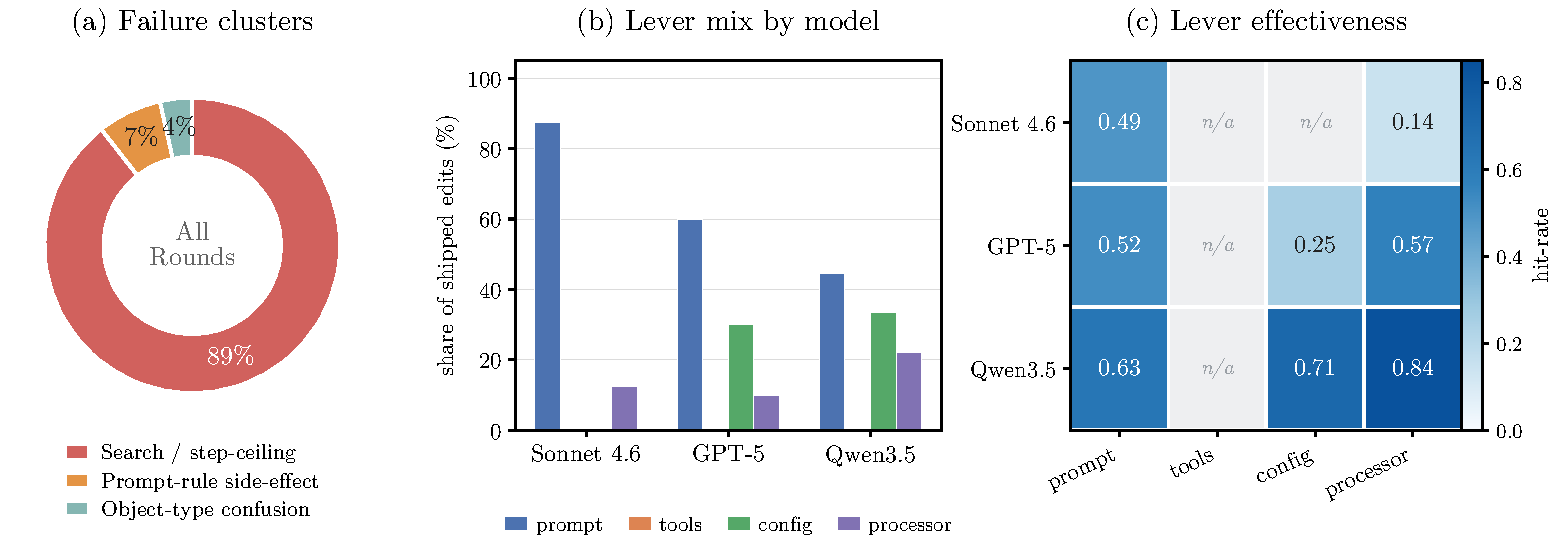
\includegraphics[width=\linewidth]{images/bench_alfworld.pdf}
\caption{ALFWorld evolution analysis (134 tasks, goal-completion).
\textbf{(a)}~Failure clusters accumulated across all rounds; search inefficiency
and the hard step-ceiling dominate, with two small clusters that evolution itself
introduced (a prompt-rule side-effect) or transiently hit (object-type
confusion). \textbf{(b)}~Lever mix by model: the strong base (Sonnet) climbs on
prompt almost alone, while weaker bases reach for more varied levers.
\textbf{(c)}~Lever effectiveness: structural levers (processor, config) are both
used more and more effective on weaker models.}
\label{fig:alfworld-detail}
\end{figure*}

% =====================================================================
\subsection{WebShop}
\label{app:webshop-detail}

WebShop is a web-interaction benchmark and the noisiest run in our suite.
Figure~\ref{fig:webshop-detail} shows its clusters, per-model logic, and
effectiveness.

\paragraph{Failure clusters and their causes.}
Panel~(a) summarizes the WebShop failure clusters accumulated across the run. Early failures are dominated by search and pagination loops, where the agent repeatedly reformulates queries or cycles through result pages without committing to a purchase. As evolution reduces these control-flow errors, the remaining failures shift toward product-selection judgment. The largest cluster, wrong product ($46\%$), occurs when the agent selects an item from the wrong category or settles on a weak match before comparing alternatives. Pagination loop failures ($21\%$) capture the remaining cases of repeated next/previous navigation without progress. Colour matching failures ($17\%$) arise when the agent mishandles shade equivalence or site-specific color labels, such as treating ``wine'' and ``red'' as incompatible. Attribute check failures ($17\%$) occur when the selected item is close to the request but fails on a required detail, such as size, sleeve length, or another unverified attribute. Overall, the cluster shift indicates that evolution first reduces navigation loops, after which the main errors concentrate in product matching and attribute verification.

\paragraph{Per-model evolution logic.}
Panel~(b) shows that prompt edits drive most of the improvement across all three models, with processor edits serving as a consistent secondary lever. This pattern matches WebShop's main control-flow failures. Prompt rules help the agent search more efficiently and commit earlier, while advisory processors reinforce these rules during execution by adding warnings when the agent begins to repeat searches or cycle through pagination. For product-selection failures, evolution introduces more targeted support: a colour-matching tool helps resolve shade-equivalence cases, and config edits help weaker models maintain context over longer shopping sessions. Overall, WebShop requires a mixed response: prompts improve high-level shopping strategy, processors reduce navigation loops, tools support attribute matching, and config edits stabilize long-session behavior.

\paragraph{Did evolution close the clusters?}
Panel~(c) shows that evolution partially reduced the WebShop failure clusters. Prompt edits were the most consistently effective lever across models, with hit-rates of $0.37$--$0.50$, while config edits helped the two weaker models maintain context over longer sessions. These changes reduced early search and pagination loops, raising performance from $60\%$ to a peak of $76\%$. The remaining clusters proved harder to close. Advisory processors produced only modest gains ($0.20$--$0.25$), so some pagination failures persisted. The colour-matching tool did not improve performance in this run ($0.0$ hit-rate), leaving the colour-matching cluster largely unchanged. Overall, WebShop benefits most from prompt and config edits, while residual navigation loops and product-judgment errors remain the main sources of instability.

\begin{figure*}[!htbp]
\centering
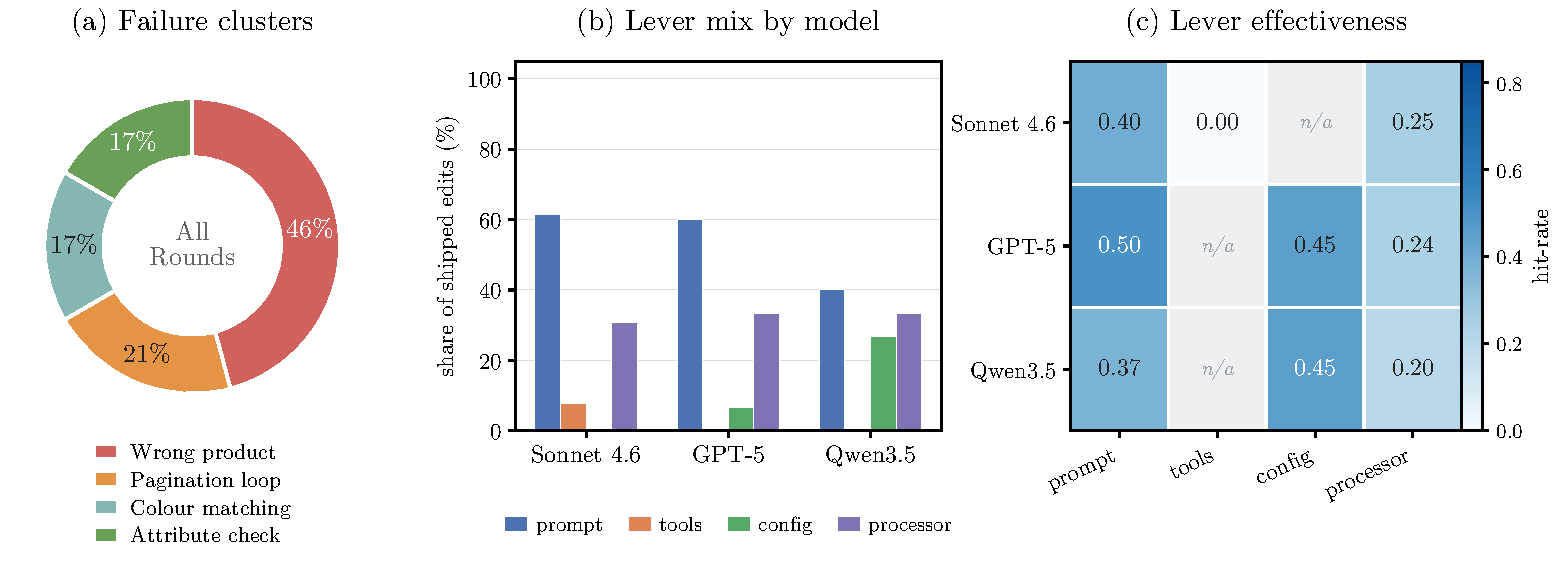
\includegraphics[width=\linewidth]{images/bench_webshop.pdf}
\caption{WebShop evolution analysis (100 sessions).
\textbf{(a)}~Failure clusters across the run, after evolution has tamed the
round-0 search/pagination loops; the residual is mostly product-choice judgment
(wrong product, colour matching, attribute check). \textbf{(b)}~Lever mix by
model: prompt carries the climb, processor is the consistent second lever.
\textbf{(c)}~Lever effectiveness; prompt and config are the productive levers,
the lone colour-matcher tool ship returned $0.0$.}
\label{fig:webshop-detail}
\end{figure*}

% =====================================================================
\subsection{$\tau^3$-Bench}
\label{app:tau3-detail}

$\tau^3$-Bench stresses multi-turn dialogue under an explicit domain policy.
Figure~\ref{fig:tau3-detail} pools the AEGIS runs across the airline, retail,
and telecom domains.

\paragraph{Failure clusters and their causes.}
Excluding harness-interrupt traces, the failures are judgment-heavy: the top two
clusters, premature / unverified action ($28\%$; committing a booking, refund,
or device fix before a precondition holds) and wrong selection / count
($24\%$), together exceed half and concern \emph{when} to commit and
\emph{what} to pick rather than mechanical execution. The remainder is
procedural (incomplete multi-step fix $16\%$, missed step / sub-task $14\%$) or
policy-related (misinterpretation $13\%$). The smallest cluster,
capability-boundary confusion ($5\%$), is $\tau^3$-specific: some telecom faults
live on the user's handset, where the agent has no device-side tool and the
failure is its treating that boundary as a missing capability.

\paragraph{Per-model evolution logic.}
Evolution is prompt-and-processor driven for every model, with zero tools edits:
the tool set is fixed and no cluster is one that a new tool could close. Sonnet 4.6
splits prompt/processor ($23/18$), GPT-5.4 ships the most balanced mix
($19/20$), and Qwen3.5-9B ships fewer overall ($14/9$). Since $\tau^3$ failures
are control-flow and judgment errors, the productive levers are prompt rules
that encode the policy's ordering constraints and processors that enforce them
mid-dialogue.

\paragraph{Did evolution close the clusters?}
Config is the sharpest lever where used (Qwen3.5 $0.67$, GPT-5.4 $0.33$ hit-rate)
but is shipped rarely; the high-volume prompt and processor levers are moderately
effective ($0.27$--$0.35$), matching the control-flow nature of the dominant
clusters. Gains track base-model headroom: GPT-5.4 starts lowest ($76.2\%$) and
gains most ($+14.5$pp), Sonnet 4.6 gains $+5.4$pp, and near-ceiling Qwen3.5-9B
only $+1.1$pp. The loop is not monotone; Sonnet's telecom run reaches $100\%$
at R4, regresses to $80.7\%$ at R7 after a sixth consecutive same-bucket edit,
then recovers to $99.1\%$ by R9 (Section~\ref{sec:exp-failure}). Overall, the
ordering-enforcing levers close the premature-action and missed-step clusters
most reliably, while wrong-selection and policy-judgment errors are the harder
residual.

\begin{figure*}[!htbp]
\centering
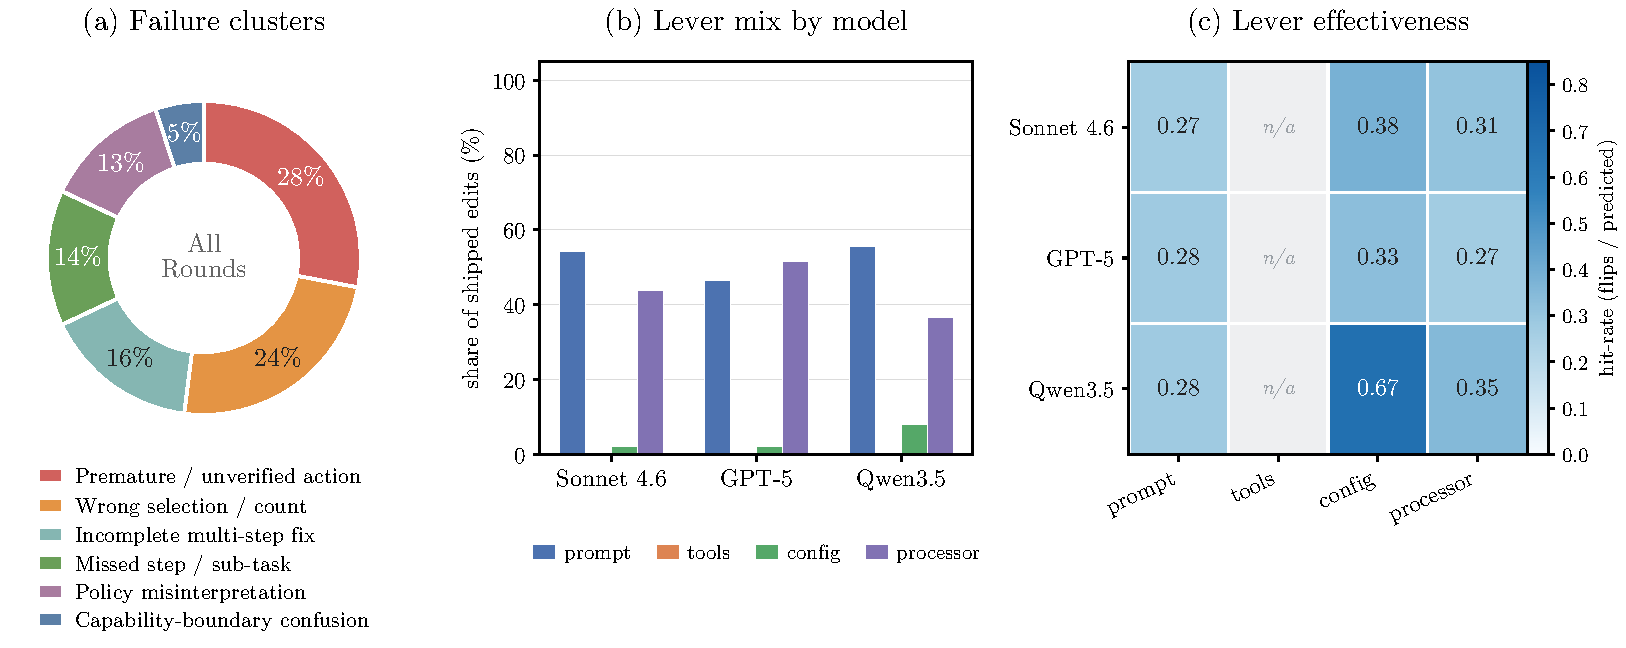
\includegraphics[width=\linewidth]{images/bench_tau3.pdf}
\caption{$\tau^3$-Bench evolution analysis, pooled over the airline, retail, and
telecom domains. \textbf{(a)}~Failure clusters from the logged digests
(harness-interrupt traces excluded); judgment errors (premature action and
wrong selection) dominate. \textbf{(b)}~Lever mix by model: prompt and
processor carry the climb, with zero tools edits since the tool set is fixed.
\textbf{(c)}~Lever effectiveness; config is sharpest where used (Qwen3.5 $0.67$)
but rare, while prompt and processor are the consistent high-volume levers.}
\label{fig:tau3-detail}
\end{figure*}

% =====================================================================
\subsection{SWE-bench Verified}
\label{app:swe-detail}

SWE-bench Verified stresses repository-level code editing. 
Figure~\ref{fig:swe-detail} shows its clusters, per-model logic, and effectiveness.

\paragraph{Failure clusters and their causes.} 

Panel~(a) summarizes the failure clusters pooled across all rounds and all three models. The dominant cluster is incomplete fix ($62\%$), where the agent reaches the right region and produces a valid patch but covers only one branch or call site while the gold patch needs several. Wrong diagnosis ($19\%$) follows, covering edits to the wrong file or abstraction level after misreading the root cause. The remaining tail is mechanical rather than cognitive: no edit attempted ($6\%$), \texttt{Edit} anchor mismatch ($5\%$), and budget exhausted ($4\%$). Notably the composition is the inverse of reward-hacking: failures are under-fixes, not gamed evaluations, because the harness applies the gold test patch before the model patch and blocks test-file writes.
  
\paragraph{Per-model evolution logic.} 

Panel~(b) shows that SWE-bench is prompt-first for every model, with the secondary lever tracking base-model strength. All three runs ship zero tools edits, since unlike GAIA the failure set has no mechanical-retrieval cluster a tool could close. Sonnet pairs prompt with an equal share of processor edits ($7$ each), using workflow nudges to shape an already-competent coder; GPT-5.4 leans hardest on prompt ($8$ ships) and uses config ($4$) to revert a harmful nudge and restructure its strategy phases; Qwen3.5 spreads its few ships across prompt, processor, and config ($6/3/3$). The shared logic is prompt-first, with structural levers recruited as the base model weakens.

\paragraph{Did evolution close the clusters?} 
Panel~(c) reveals a sharp capability floor. For the strong models the productive levers genuinely close failures: GPT-5.4's config edits reach $0.48$ and prompt $0.39$, while Sonnet's prompt and processor levers both land at $0.40$. For Qwen3.5-9B every lever collapses to near-zero (prompt $0.05$, config $0.05$, processor $0.06$), an order of magnitude lower, because the $9$B base cannot execute the predicted fixes. The same loop that lifts GPT-5.4 from $45\%$ to a $64\%$ peak and stabilizes Sonnet near $87\%$ yields only noise on Qwen3.5 (peak $42\%$, zero durable gains). Overall SWE-bench improves through prompt edits that broaden fix scope and config edits that restore workflow pacing, but only for models strong enough to act on them.

\begin{figure*}[!htbp]
\centering
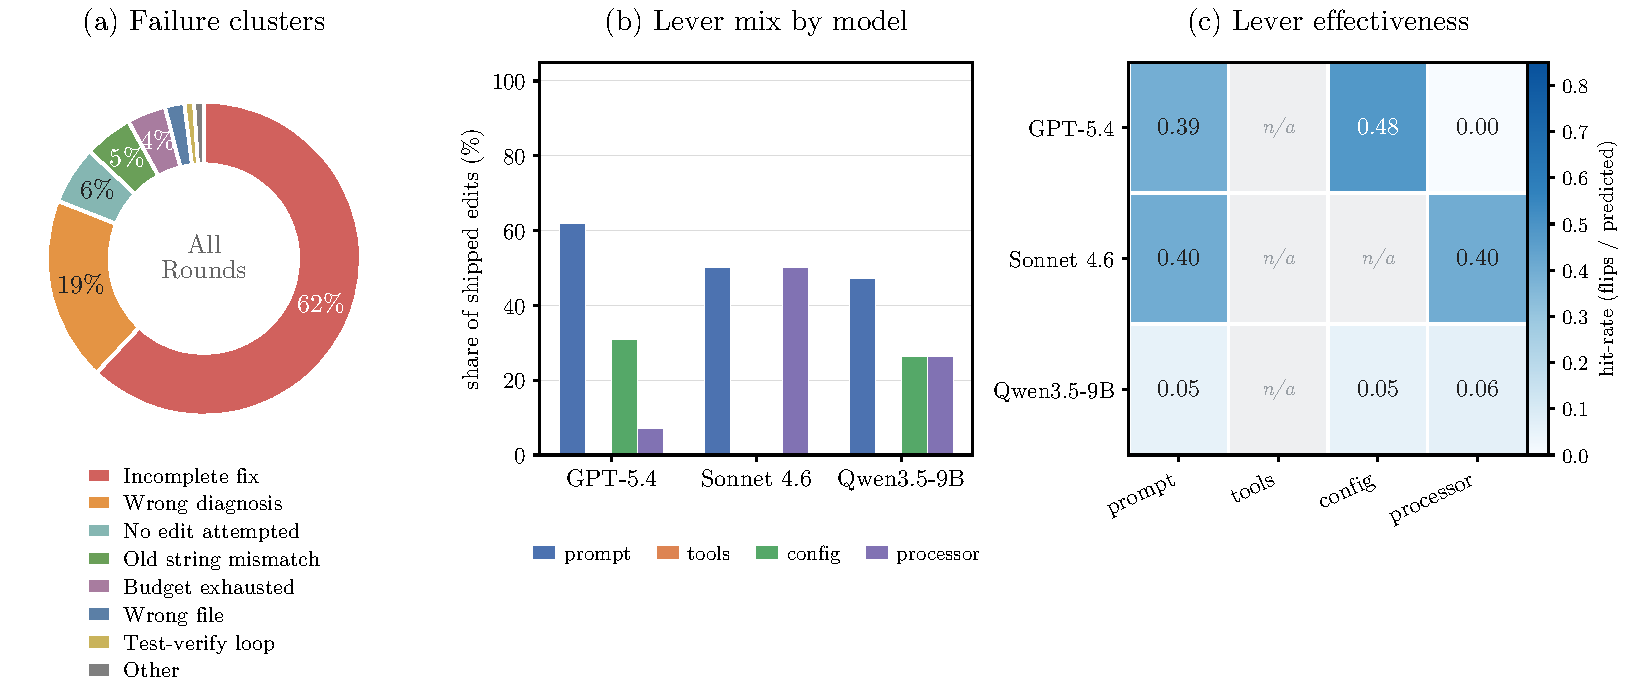
\includegraphics[width=\linewidth]{images/bench_swebench.pdf}
\caption{SWE-bench Verified evolution analysis ($55$ tasks, resolved-rate).
\textbf{(a)}~Failure clusters pooled across all rounds and all three task models;
incomplete fix and wrong diagnosis dominate, while the mechanical tail (no-edit,
anchor mismatch, budget) is residual; failures are under-fixes, not gamed
evaluations. \textbf{(b)}~Lever mix by model: every run is prompt-first and ships
zero tools edits, with the secondary lever shifting from processor (Sonnet) to
config (GPT-5.4) to a varied mix (Qwen3.5). \textbf{(c)}~Lever effectiveness as
hit-rate (tasks flipped / predicted); strong models reach $0.39$--$0.48$ on their
productive levers, whereas every Qwen3.5-9B lever collapses to $\approx0.05$, a
capability floor below which evolution cannot compound.}
\label{fig:swe-detail}
\end{figure*}

\section{Reproducibility and Artifacts}
\label{app:artifacts}

\subsection{Per-Run Directory Layout}
Each evolution run writes a self-describing directory. The layout below lets a
reader reconstruct any decision in this paper from the logged artifacts.

\begin{promptfile}{runs/<run\_name>/ (per-run artifact layout)}
runs/<run_name>/
|-- INDEX.md            # human-readable index of the run
|-- journal.md          # first-person memo, one entry per round
|-- curves.json         # per-round pass-rate trajectory
|-- scoreboard.json     # ships + per-bucket reputation
|-- audit.jsonl         # structured event log (stage / gate / commit)
|-- data/
|   |-- task_history.jsonl      # one line per (round, task)
|   |-- ship_outcomes.json      # one entry per historical ship
|   `-- rejected_candidates.jsonl
`-- R<n>/                        # per-round artifacts
    |-- landscape.md             # Planner cross-trace synthesis
    |-- candidates/C-R<n>-NN.md  # Evolver change manifests (K per round)
    |-- applied/C-R<n>-NN/       # applied config + asset files
    |-- decision.md              # Critic ship / no_op decision
    |-- verdicts/V-C-R<n>-NN.md  # per-candidate verdicts
    |-- regressions.md           # tasks worsened vs R<n-1>
    |-- digests/*.md             # per-task failure analysis
    `-- trajectories/*.jsonl     # raw rollouts
\end{promptfile}

